\documentclass{article}
\usepackage[utf8]{inputenc}
\usepackage{tikz}
\usepackage{amssymb}
\usepackage{amsmath}
\usepackage{amssymb}

\begin{document}

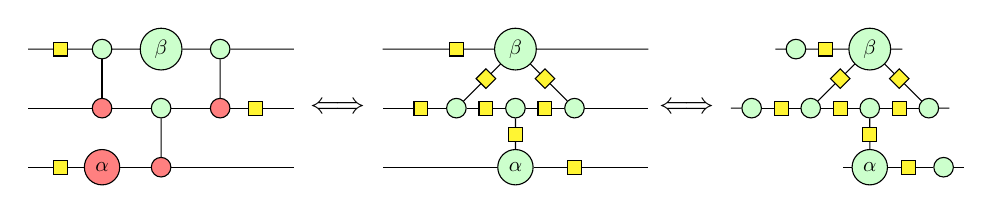
\begin{tikzpicture}[scale=0.75, transform shape]
    \node[shape=circle,draw=black,fill=white!50!red] (A) at (0,0) {$\alpha$};
    \node[shape=circle,draw=black,fill=white!50!red] (B) at (1,0) {};
    \node[shape=circle,draw=black,fill=white!80!green] (C) at (1,1) {};
    \node[shape=circle,draw=black,fill=white!80!green] (D) at (1,2) {$\beta$};
    \node[shape=circle,draw=black,fill=white!50!red] (E) at (0,1) {};
    \node[shape=circle,draw=black,fill=white!80!green] (F) at (0,2) {};
    \node[shape=circle,draw=black,fill=white!50!red] (G) at (2,1) {};
    \node[shape=circle,draw=black,fill=white!80!green] (H) at (2,2) {};
    \coordinate (F2) at (-1.25,2);
    \coordinate (E2) at (-1.25,1);
    \coordinate (A2) at (-1.25,0);
    \coordinate (H2) at (3.25,2);
    \coordinate (G2) at (3.25,1);
    \coordinate (B2) at (3.25,0);
    \draw[-] (B) -- (C);
    \draw[-] (A) -- (B);
    \draw[-] (F) -- (D);
    \draw[-] (E) -- (F);
    \draw[-] (E) -- (C);
    \draw[-] (G) -- (H);
    \draw[-] (C) -- (G);
    \draw[-] (D) -- (H);
    \draw[-] (F) -- (F2);
    \draw[-] (E) -- (E2);
    \draw[-] (A) -- (A2);
    \draw[-] (H) -- (H2);
    \draw[-] (G) -- (G2);
    \draw[-] (B) -- (B2);
    \node[shape=rectangle,draw=black,fill=white!20!yellow] (h) at (2.6,1) {};
    \node[shape=rectangle,draw=black,fill=white!20!yellow] (h) at (-0.7,2) {};
    \node[shape=rectangle,draw=black,fill=white!20!yellow] (h) at (-0.7,0) {};
    \node[shape=rectangle,draw=white] (eq) at (4,1) {\Large $\Longleftrightarrow$};
    
    \node[shape=circle,draw=black,fill=white!80!green] (B) at (7,0) {$\alpha$};
    \node[shape=circle,draw=black,fill=white!80!green] (C) at (7,1) {};
    \node[shape=circle,draw=black,fill=white!80!green] (D) at (7,2) {$\beta$};
    \node[shape=circle,draw=black,fill=white!80!green] (E) at (6,1) {};
    \node[shape=circle,draw=black,fill=white!80!green] (G) at (8,1) {};
    \coordinate (F2) at (4.75,2);
    \coordinate (E2) at (4.75,1);
    \coordinate (A2) at (4.75,0);
    \coordinate (H2) at (9.25,2);
    \coordinate (G2) at (9.25,1);
    \coordinate (B2) at (9.25,0);
    \draw[-] (B) -- (C);
    \draw[-] (E) -- (D);
    \draw[-] (E) -- (C);
    \draw[-] (G) -- (D);
    \draw[-] (C) -- (G);
    \draw[-] (D) -- (F2);
    \draw[-] (E) -- (E2);
    \draw[-] (B) -- (A2);
    \draw[-] (D) -- (H2);
    \draw[-] (G) -- (G2);
    \draw[-] (B) -- (B2);
    \node[shape=rectangle,draw=black,fill=white!20!yellow,rotate=45] (h) at (6.5,1.5) {};
    \node[shape=rectangle,draw=black,fill=white!20!yellow,rotate=45] (h) at (7.5,1.5) {};
    \node[shape=rectangle,draw=black,fill=white!20!yellow] (h) at (6,2) {};
    \node[shape=rectangle,draw=black,fill=white!20!yellow] (h) at (5.4,1) {};
    \node[shape=rectangle,draw=black,fill=white!20!yellow] (h) at (6.5,1) {};
    \node[shape=rectangle,draw=black,fill=white!20!yellow] (h) at (7.5,1) {};
    \node[shape=rectangle,draw=black,fill=white!20!yellow] (h) at (8,0) {};
    \node[shape=rectangle,draw=black,fill=white!20!yellow] (h) at (7,0.55) {}; 

    \node[shape=rectangle,draw=white] (eq) at (9.9,1) {\Large $\Longleftrightarrow$};

    \node[shape=circle,draw=black,fill=white!80!green] (B) at (13,0) {$\alpha$};
    \node[shape=circle,draw=black,fill=white!80!green] (C) at (13,1) {};
    \node[shape=circle,draw=black,fill=white!80!green] (D) at (13,2) {$\beta$};
    \node[shape=circle,draw=black,fill=white!80!green] (E) at (12,1) {};
    \node[shape=circle,draw=black,fill=white!80!green] (G) at (14,1) {};
    \node[shape=circle,draw=black,fill=white!80!green] (F2) at (11.75,2) {};
    \node[shape=circle,draw=black,fill=white!80!green] (E2) at (11,1) {};
    \node[shape=circle,draw=black,fill=white!80!green] (B2) at (14.25,0) {};
    \draw[-] (B) -- (C);
    \draw[-] (E) -- (D);
    \draw[-] (E) -- (C);
    \draw[-] (G) -- (D);
    \draw[-] (C) -- (G);
    \draw[-] (D) -- (F2);
    \draw[-] (E) -- (E2);
    \draw[-] (B) -- (B2);
    \draw[-] (F2) -- (11.4,2);
    \draw[-] (E2) -- (10.65,1);
    \draw[-] (B2) -- (14.6,0);
    \draw[-] (B) -- (12.55,0);
    \draw[-] (G) -- (14.35,1);
    \draw[-] (D) -- (13.55,2);

    \node[shape=rectangle,draw=black,fill=white!20!yellow,rotate=45] (h) at (12.5,1.5) {};
    \node[shape=rectangle,draw=black,fill=white!20!yellow,rotate=45] (h) at (13.5,1.5) {};
    \node[shape=rectangle,draw=black,fill=white!20!yellow] (h) at (12.25,2) {};
    \node[shape=rectangle,draw=black,fill=white!20!yellow] (h) at (11.5,1) {};
    \node[shape=rectangle,draw=black,fill=white!20!yellow] (h) at (12.5,1) {};
    \node[shape=rectangle,draw=black,fill=white!20!yellow] (h) at (13.5,1) {};
    \node[shape=rectangle,draw=black,fill=white!20!yellow] (h) at (13.65,0) {};
    \node[shape=rectangle,draw=black,fill=white!20!yellow] (h) at (13,0.55) {}; 
\end{tikzpicture}

\end{document}